% GNUPLOT: LaTeX picture with Postscript
\begingroup
  \makeatletter
  \providecommand\color[2][]{%
    \GenericError{(gnuplot) \space\space\space\@spaces}{%
      Package color not loaded in conjunction with
      terminal option `colourtext'%
    }{See the gnuplot documentation for explanation.%
    }{Either use 'blacktext' in gnuplot or load the package
      color.sty in LaTeX.}%
    \renewcommand\color[2][]{}%
  }%
  \providecommand\includegraphics[2][]{%
    \GenericError{(gnuplot) \space\space\space\@spaces}{%
      Package graphicx or graphics not loaded%
    }{See the gnuplot documentation for explanation.%
    }{The gnuplot epslatex terminal needs graphicx.sty or graphics.sty.}%
    \renewcommand\includegraphics[2][]{}%
  }%
  \providecommand\rotatebox[2]{#2}%
  \@ifundefined{ifGPcolor}{%
    \newif\ifGPcolor
    \GPcolortrue
  }{}%
  \@ifundefined{ifGPblacktext}{%
    \newif\ifGPblacktext
    \GPblacktextfalse
  }{}%
  % define a \g@addto@macro without @ in the name:
  \let\gplgaddtomacro\g@addto@macro
  % define empty templates for all commands taking text:
  \gdef\gplbacktext{}%
  \gdef\gplfronttext{}%
  \makeatother
  \ifGPblacktext
    % no textcolor at all
    \def\colorrgb#1{}%
    \def\colorgray#1{}%
  \else
    % gray or color?
    \ifGPcolor
      \def\colorrgb#1{\color[rgb]{#1}}%
      \def\colorgray#1{\color[gray]{#1}}%
      \expandafter\def\csname LTw\endcsname{\color{white}}%
      \expandafter\def\csname LTb\endcsname{\color{black}}%
      \expandafter\def\csname LTa\endcsname{\color{black}}%
      \expandafter\def\csname LT0\endcsname{\color[rgb]{1,0,0}}%
      \expandafter\def\csname LT1\endcsname{\color[rgb]{0,1,0}}%
      \expandafter\def\csname LT2\endcsname{\color[rgb]{0,0,1}}%
      \expandafter\def\csname LT3\endcsname{\color[rgb]{1,0,1}}%
      \expandafter\def\csname LT4\endcsname{\color[rgb]{0,1,1}}%
      \expandafter\def\csname LT5\endcsname{\color[rgb]{1,1,0}}%
      \expandafter\def\csname LT6\endcsname{\color[rgb]{0,0,0}}%
      \expandafter\def\csname LT7\endcsname{\color[rgb]{1,0.3,0}}%
      \expandafter\def\csname LT8\endcsname{\color[rgb]{0.5,0.5,0.5}}%
    \else
      % gray
      \def\colorrgb#1{\color{black}}%
      \def\colorgray#1{\color[gray]{#1}}%
      \expandafter\def\csname LTw\endcsname{\color{white}}%
      \expandafter\def\csname LTb\endcsname{\color{black}}%
      \expandafter\def\csname LTa\endcsname{\color{black}}%
      \expandafter\def\csname LT0\endcsname{\color{black}}%
      \expandafter\def\csname LT1\endcsname{\color{black}}%
      \expandafter\def\csname LT2\endcsname{\color{black}}%
      \expandafter\def\csname LT3\endcsname{\color{black}}%
      \expandafter\def\csname LT4\endcsname{\color{black}}%
      \expandafter\def\csname LT5\endcsname{\color{black}}%
      \expandafter\def\csname LT6\endcsname{\color{black}}%
      \expandafter\def\csname LT7\endcsname{\color{black}}%
      \expandafter\def\csname LT8\endcsname{\color{black}}%
    \fi
  \fi
  \setlength{\unitlength}{0.0500bp}%
  \begin{picture}(19274.00,14740.00)%
    \gplgaddtomacro\gplbacktext{%
      \colorrgb{0.50,0.50,0.50}%
      \put(1405,10229){\makebox(0,0)[r]{\strut{}\footnotesize $0$}}%
      \colorrgb{0.50,0.50,0.50}%
      \put(1405,10963){\makebox(0,0)[r]{\strut{}\footnotesize $0.2$}}%
      \colorrgb{0.50,0.50,0.50}%
      \put(1405,11696){\makebox(0,0)[r]{\strut{}\footnotesize $0.4$}}%
      \colorrgb{0.50,0.50,0.50}%
      \put(1405,12429){\makebox(0,0)[r]{\strut{}\footnotesize $0.6$}}%
      \colorrgb{0.50,0.50,0.50}%
      \put(1405,13162){\makebox(0,0)[r]{\strut{}\footnotesize $0.8$}}%
      \colorrgb{0.50,0.50,0.50}%
      \put(1405,13896){\makebox(0,0)[r]{\strut{}\footnotesize $1$}}%
      \colorrgb{0.50,0.50,0.50}%
      \put(1584,9779){\makebox(0,0){\strut{}}}%
      \colorrgb{0.50,0.50,0.50}%
      \put(3194,9779){\makebox(0,0){\strut{}}}%
      \colorrgb{0.50,0.50,0.50}%
      \put(4805,9779){\makebox(0,0){\strut{}}}%
      \colorrgb{0.50,0.50,0.50}%
      \put(6415,9779){\makebox(0,0){\strut{}}}%
      \colorrgb{0.50,0.50,0.50}%
      \put(8026,9779){\makebox(0,0){\strut{}}}%
      \colorrgb{0.50,0.50,0.50}%
      \put(9636,9779){\makebox(0,0){\strut{}}}%
      \csname LTb\endcsname%
      \put(371,12062){\rotatebox{-270}{\makebox(0,0){\strut{}$| H_{\mathrm{frac}} |$}}}%
    }%
    \gplgaddtomacro\gplfronttext{%
      \csname LTb\endcsname%
      \put(2973,12649){\makebox(0,0)[r]{\strut{}\footnotesize $N=0$}}%
      \csname LTb\endcsname%
      \put(2973,12209){\makebox(0,0)[r]{\strut{}\footnotesize $N=1$}}%
      \csname LTb\endcsname%
      \put(2973,11769){\makebox(0,0)[r]{\strut{}\footnotesize $N=2$}}%
      \csname LTb\endcsname%
      \put(2973,11329){\makebox(0,0)[r]{\strut{}\footnotesize $N=3$}}%
      \csname LTb\endcsname%
      \put(2973,10889){\makebox(0,0)[r]{\strut{}\footnotesize $N=4$}}%
      \csname LTb\endcsname%
      \put(2973,10449){\makebox(0,0)[r]{\strut{}\footnotesize $N=5$}}%
      \csname LTb\endcsname%
      \put(5610,14281){\makebox(0,0){\strut{}\small Lagrange Filter for $d_{\mathrm{frac}} = 0.5$}}%
    }%
    \gplgaddtomacro\gplbacktext{%
      \colorrgb{0.50,0.50,0.50}%
      \put(1405,5536){\makebox(0,0)[r]{\strut{}\footnotesize $0$}}%
      \colorrgb{0.50,0.50,0.50}%
      \put(1405,6270){\makebox(0,0)[r]{\strut{}\footnotesize $0.2$}}%
      \colorrgb{0.50,0.50,0.50}%
      \put(1405,7003){\makebox(0,0)[r]{\strut{}\footnotesize $0.4$}}%
      \colorrgb{0.50,0.50,0.50}%
      \put(1405,7736){\makebox(0,0)[r]{\strut{}\footnotesize $0.6$}}%
      \colorrgb{0.50,0.50,0.50}%
      \put(1405,8469){\makebox(0,0)[r]{\strut{}\footnotesize $0.8$}}%
      \colorrgb{0.50,0.50,0.50}%
      \put(1405,9203){\makebox(0,0)[r]{\strut{}\footnotesize $1$}}%
      \colorrgb{0.50,0.50,0.50}%
      \put(1584,5086){\makebox(0,0){\strut{}}}%
      \colorrgb{0.50,0.50,0.50}%
      \put(3194,5086){\makebox(0,0){\strut{}}}%
      \colorrgb{0.50,0.50,0.50}%
      \put(4805,5086){\makebox(0,0){\strut{}}}%
      \colorrgb{0.50,0.50,0.50}%
      \put(6415,5086){\makebox(0,0){\strut{}}}%
      \colorrgb{0.50,0.50,0.50}%
      \put(8026,5086){\makebox(0,0){\strut{}}}%
      \colorrgb{0.50,0.50,0.50}%
      \put(9636,5086){\makebox(0,0){\strut{}}}%
      \csname LTb\endcsname%
      \put(371,7369){\rotatebox{-270}{\makebox(0,0){\strut{}$| H_{\mathrm{frac}} |$}}}%
    }%
    \gplgaddtomacro\gplfronttext{%
      \colorrgb{0.65,0.34,0.16}%
      \put(9636,8836){\makebox(0,0)[r]{\strut{}\footnotesize $N=1,2,3,4,5,6$}}%
      \csname LTb\endcsname%
      \put(5610,9588){\makebox(0,0){\strut{}\small Thiran Filter for $d_{\mathrm{frac}} = 0.5$}}%
    }%
    \gplgaddtomacro\gplbacktext{%
      \colorrgb{0.50,0.50,0.50}%
      \put(1405,843){\makebox(0,0)[r]{\strut{}\footnotesize $0$}}%
      \colorrgb{0.50,0.50,0.50}%
      \put(1405,1577){\makebox(0,0)[r]{\strut{}\footnotesize $0.2$}}%
      \colorrgb{0.50,0.50,0.50}%
      \put(1405,2310){\makebox(0,0)[r]{\strut{}\footnotesize $0.4$}}%
      \colorrgb{0.50,0.50,0.50}%
      \put(1405,3043){\makebox(0,0)[r]{\strut{}\footnotesize $0.6$}}%
      \colorrgb{0.50,0.50,0.50}%
      \put(1405,3776){\makebox(0,0)[r]{\strut{}\footnotesize $0.8$}}%
      \colorrgb{0.50,0.50,0.50}%
      \put(1405,4510){\makebox(0,0)[r]{\strut{}\footnotesize $1$}}%
      \colorrgb{0.50,0.50,0.50}%
      \put(1584,393){\makebox(0,0){\strut{}\footnotesize $0$}}%
      \colorrgb{0.50,0.50,0.50}%
      \put(3194,393){\makebox(0,0){\strut{}\footnotesize $0.1$}}%
      \colorrgb{0.50,0.50,0.50}%
      \put(4805,393){\makebox(0,0){\strut{}\footnotesize $0.2$}}%
      \colorrgb{0.50,0.50,0.50}%
      \put(6415,393){\makebox(0,0){\strut{}\footnotesize $0.3$}}%
      \colorrgb{0.50,0.50,0.50}%
      \put(8026,393){\makebox(0,0){\strut{}\footnotesize $0.4$}}%
      \colorrgb{0.50,0.50,0.50}%
      \put(9636,393){\makebox(0,0){\strut{}\footnotesize $0.5$}}%
      \csname LTb\endcsname%
      \put(371,2676){\rotatebox{-270}{\makebox(0,0){\strut{}$| H_{\mathrm{frac}} |$}}}%
      \put(5610,-157){\makebox(0,0){\strut{}$f / f_s$}}%
    }%
    \gplgaddtomacro\gplfronttext{%
      \csname LTb\endcsname%
      \put(4029,3630){\makebox(0,0)[r]{\strut{}\footnotesize $d_{\mathrm{frac}}=0.00$}}%
      \csname LTb\endcsname%
      \put(4029,3190){\makebox(0,0)[r]{\strut{}\footnotesize $d_{\mathrm{frac}}=0.05$}}%
      \csname LTb\endcsname%
      \put(4029,2750){\makebox(0,0)[r]{\strut{}\footnotesize $d_{\mathrm{frac}}=0.10$}}%
      \csname LTb\endcsname%
      \put(4029,2310){\makebox(0,0)[r]{\strut{}\footnotesize $d_{\mathrm{frac}}=0.15$}}%
      \csname LTb\endcsname%
      \put(4029,1870){\makebox(0,0)[r]{\strut{}\footnotesize $d_{\mathrm{frac}}=0.20$}}%
      \csname LTb\endcsname%
      \put(4029,1430){\makebox(0,0)[r]{\strut{}\footnotesize $d_{\mathrm{frac}}=0.25$}}%
      \csname LTb\endcsname%
      \put(5610,4895){\makebox(0,0){\strut{}\small Upsampling ($R=2$) + Lagrange ($N=1$)}}%
    }%
    \gplgaddtomacro\gplbacktext{%
      \colorrgb{0.50,0.50,0.50}%
      \put(11042,10229){\makebox(0,0)[r]{\strut{}\footnotesize $0$}}%
      \colorrgb{0.50,0.50,0.50}%
      \put(11042,10963){\makebox(0,0)[r]{\strut{}\footnotesize $0.1$}}%
      \colorrgb{0.50,0.50,0.50}%
      \put(11042,11696){\makebox(0,0)[r]{\strut{}\footnotesize $0.2$}}%
      \colorrgb{0.50,0.50,0.50}%
      \put(11042,12429){\makebox(0,0)[r]{\strut{}\footnotesize $0.3$}}%
      \colorrgb{0.50,0.50,0.50}%
      \put(11042,13162){\makebox(0,0)[r]{\strut{}\footnotesize $0.4$}}%
      \colorrgb{0.50,0.50,0.50}%
      \put(11042,13896){\makebox(0,0)[r]{\strut{}\footnotesize $0.5$}}%
      \colorrgb{0.50,0.50,0.50}%
      \put(11221,9779){\makebox(0,0){\strut{}}}%
      \colorrgb{0.50,0.50,0.50}%
      \put(12831,9779){\makebox(0,0){\strut{}}}%
      \colorrgb{0.50,0.50,0.50}%
      \put(14442,9779){\makebox(0,0){\strut{}}}%
      \colorrgb{0.50,0.50,0.50}%
      \put(16052,9779){\makebox(0,0){\strut{}}}%
      \colorrgb{0.50,0.50,0.50}%
      \put(17663,9779){\makebox(0,0){\strut{}}}%
      \colorrgb{0.50,0.50,0.50}%
      \put(19273,9779){\makebox(0,0){\strut{}}}%
      \csname LTb\endcsname%
      \put(10008,12062){\rotatebox{-270}{\makebox(0,0){\strut{}$\tau_{\mathrm ph}/$ samples}}}%
      \put(15247,9713){\makebox(0,0){\strut{}}}%
    }%
    \gplgaddtomacro\gplfronttext{%
      \colorrgb{0.89,0.10,0.11}%
      \put(12026,10596){\makebox(0,0)[l]{\strut{}\footnotesize $N=0$}}%
      \colorrgb{0.65,0.34,0.16}%
      \put(19273,13529){\makebox(0,0)[r]{\strut{}\footnotesize $N=1,3,5$}}%
      \colorrgb{0.30,0.69,0.29}%
      \put(16857,11696){\makebox(0,0)[r]{\strut{}\footnotesize $N=2$}}%
      \colorrgb{1.00,0.50,0.00}%
      \put(17663,12796){\makebox(0,0)[l]{\strut{}\footnotesize $N=4$}}%
      \csname LTb\endcsname%
      \put(15247,14281){\makebox(0,0){\strut{}\small Lagrange Filter for $d_{\mathrm{frac}} = 0.5$}}%
    }%
    \gplgaddtomacro\gplbacktext{%
      \colorrgb{0.50,0.50,0.50}%
      \put(11042,5536){\makebox(0,0)[r]{\strut{}\footnotesize $0$}}%
      \colorrgb{0.50,0.50,0.50}%
      \put(11042,6270){\makebox(0,0)[r]{\strut{}\footnotesize $0.1$}}%
      \colorrgb{0.50,0.50,0.50}%
      \put(11042,7003){\makebox(0,0)[r]{\strut{}\footnotesize $0.2$}}%
      \colorrgb{0.50,0.50,0.50}%
      \put(11042,7736){\makebox(0,0)[r]{\strut{}\footnotesize $0.3$}}%
      \colorrgb{0.50,0.50,0.50}%
      \put(11042,8469){\makebox(0,0)[r]{\strut{}\footnotesize $0.4$}}%
      \colorrgb{0.50,0.50,0.50}%
      \put(11042,9203){\makebox(0,0)[r]{\strut{}\footnotesize $0.5$}}%
      \colorrgb{0.50,0.50,0.50}%
      \put(11221,5086){\makebox(0,0){\strut{}}}%
      \colorrgb{0.50,0.50,0.50}%
      \put(12831,5086){\makebox(0,0){\strut{}}}%
      \colorrgb{0.50,0.50,0.50}%
      \put(14442,5086){\makebox(0,0){\strut{}}}%
      \colorrgb{0.50,0.50,0.50}%
      \put(16052,5086){\makebox(0,0){\strut{}}}%
      \colorrgb{0.50,0.50,0.50}%
      \put(17663,5086){\makebox(0,0){\strut{}}}%
      \colorrgb{0.50,0.50,0.50}%
      \put(19273,5086){\makebox(0,0){\strut{}}}%
      \csname LTb\endcsname%
      \put(10008,7369){\rotatebox{-270}{\makebox(0,0){\strut{}$\tau_{\mathrm ph}/$ samples}}}%
      \put(15247,5020){\makebox(0,0){\strut{}}}%
    }%
    \gplgaddtomacro\gplfronttext{%
      \csname LTb\endcsname%
      \put(12610,7956){\makebox(0,0)[r]{\strut{}\footnotesize $N=0$}}%
      \csname LTb\endcsname%
      \put(12610,7516){\makebox(0,0)[r]{\strut{}\footnotesize $N=1$}}%
      \csname LTb\endcsname%
      \put(12610,7076){\makebox(0,0)[r]{\strut{}\footnotesize $N=2$}}%
      \csname LTb\endcsname%
      \put(12610,6636){\makebox(0,0)[r]{\strut{}\footnotesize $N=3$}}%
      \csname LTb\endcsname%
      \put(12610,6196){\makebox(0,0)[r]{\strut{}\footnotesize $N=4$}}%
      \csname LTb\endcsname%
      \put(12610,5756){\makebox(0,0)[r]{\strut{}\footnotesize $N=5$}}%
      \csname LTb\endcsname%
      \put(15247,9588){\makebox(0,0){\strut{}\small Thiran Filter for $d_{\mathrm{frac}} = 0.5$}}%
    }%
    \gplgaddtomacro\gplbacktext{%
      \colorrgb{0.50,0.50,0.50}%
      \put(11042,843){\makebox(0,0)[r]{\strut{}\footnotesize $0$}}%
      \colorrgb{0.50,0.50,0.50}%
      \put(11042,1577){\makebox(0,0)[r]{\strut{}\footnotesize $0.1$}}%
      \colorrgb{0.50,0.50,0.50}%
      \put(11042,2310){\makebox(0,0)[r]{\strut{}\footnotesize $0.2$}}%
      \colorrgb{0.50,0.50,0.50}%
      \put(11042,3043){\makebox(0,0)[r]{\strut{}\footnotesize $0.3$}}%
      \colorrgb{0.50,0.50,0.50}%
      \put(11042,3776){\makebox(0,0)[r]{\strut{}\footnotesize $0.4$}}%
      \colorrgb{0.50,0.50,0.50}%
      \put(11042,4510){\makebox(0,0)[r]{\strut{}\footnotesize $0.5$}}%
      \colorrgb{0.50,0.50,0.50}%
      \put(11221,393){\makebox(0,0){\strut{}\footnotesize $0$}}%
      \colorrgb{0.50,0.50,0.50}%
      \put(12831,393){\makebox(0,0){\strut{}\footnotesize $0.1$}}%
      \colorrgb{0.50,0.50,0.50}%
      \put(14442,393){\makebox(0,0){\strut{}\footnotesize $0.2$}}%
      \colorrgb{0.50,0.50,0.50}%
      \put(16052,393){\makebox(0,0){\strut{}\footnotesize $0.3$}}%
      \colorrgb{0.50,0.50,0.50}%
      \put(17663,393){\makebox(0,0){\strut{}\footnotesize $0.4$}}%
      \colorrgb{0.50,0.50,0.50}%
      \put(19273,393){\makebox(0,0){\strut{}\footnotesize $0.5$}}%
      \csname LTb\endcsname%
      \put(10008,2676){\rotatebox{-270}{\makebox(0,0){\strut{}$\tau_{\mathrm ph}/$ samples}}}%
      \put(15247,-157){\makebox(0,0){\strut{}$f / f_s$}}%
    }%
    \gplgaddtomacro\gplfronttext{%
      \csname LTb\endcsname%
      \put(13666,3923){\makebox(0,0)[r]{\strut{}\footnotesize $d_{\mathrm{frac}}=0.00$}}%
      \csname LTb\endcsname%
      \put(13666,3483){\makebox(0,0)[r]{\strut{}\footnotesize $d_{\mathrm{frac}}=0.05$}}%
      \csname LTb\endcsname%
      \put(13666,3043){\makebox(0,0)[r]{\strut{}\footnotesize $d_{\mathrm{frac}}=0.10$}}%
      \csname LTb\endcsname%
      \put(17557,3923){\makebox(0,0)[r]{\strut{}\footnotesize $d_{\mathrm{frac}}=0.15$}}%
      \csname LTb\endcsname%
      \put(17557,3483){\makebox(0,0)[r]{\strut{}\footnotesize $d_{\mathrm{frac}}=0.20$}}%
      \csname LTb\endcsname%
      \put(17557,3043){\makebox(0,0)[r]{\strut{}\footnotesize $d_{\mathrm{frac}}=0.25$}}%
      \csname LTb\endcsname%
      \put(15247,4895){\makebox(0,0){\strut{}\small Upsampling ($R=2$) + Lagrange ($N=1$)}}%
    }%
    \gplbacktext
    \put(0,0){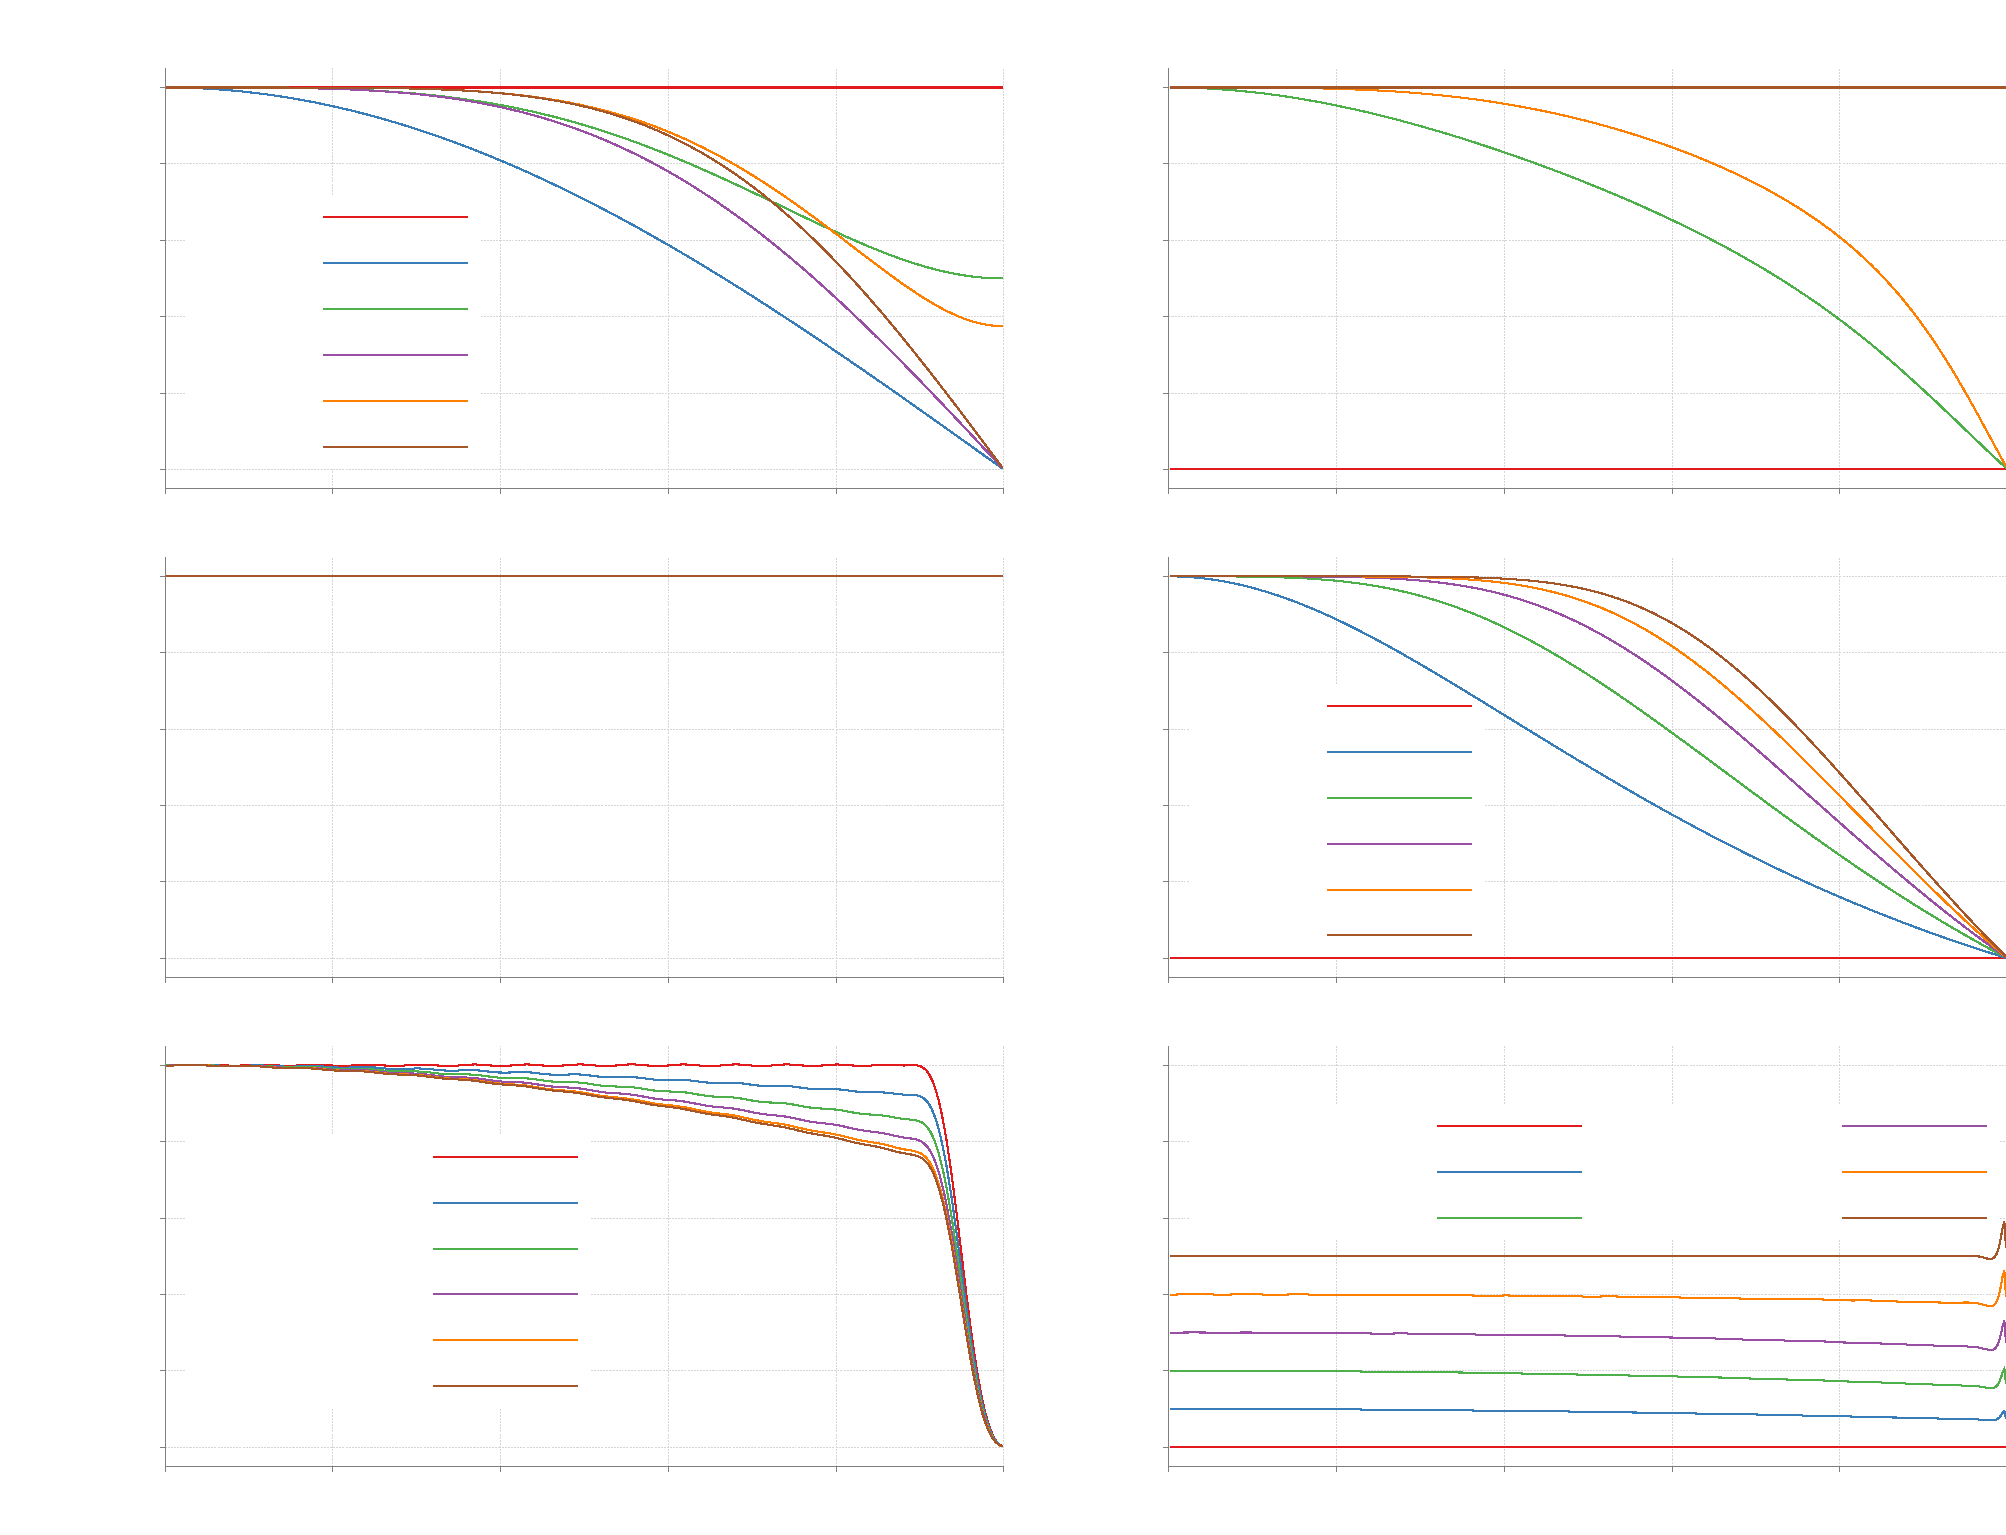
\includegraphics{fig}}%
    \gplfronttext
  \end{picture}%
\endgroup
